%
% Complete documentation on the extended LaTeX markup used for Insight
% documentation is available in ``Documenting Insight'', which is part
% of the standard documentation for Insight.  It may be found online
% at:
%
%     http://www.itk.org/

\documentclass{InsightArticle}


%%%%%%%%%%%%%%%%%%%%%%%%%%%%%%%%%%%%%%%%%%%%%%%%%%%%%%%%%%%%%%%%%%
%
%  hyperref should be the last package to be loaded.
%
%%%%%%%%%%%%%%%%%%%%%%%%%%%%%%%%%%%%%%%%%%%%%%%%%%%%%%%%%%%%%%%%%%
\usepackage[dvips,
bookmarks,
bookmarksopen,
backref,
colorlinks,linkcolor={blue},citecolor={blue},urlcolor={blue},
]{hyperref}
\usepackage{graphicx}
\usepackage{listings}
\usepackage{subfigure}
\title{Finding regional extrema - methods\\ and performance}

%\release{1.00}

\author{Richard Beare{$^1$} {\small{and}} Ga\"etan Lehmann{$^2$}}
\authoraddress{{$^1$}Department of Medicine, Moansh University, Australia.\\ 
{$^2$}Unit\'e de Biologie du D\'eveloppement et de la Reproduction, Institut National de la Recherche Agronomique, 78350 Jouy-en-Josas, France}


\begin{document}
\maketitle

\ifhtml
\chapter*{Front Matter\label{front}}
\fi

\begin{abstract}
\noindent
Finding regional extrema of images is an important step in a number of
morphological algorithms, such as some versions of the watershed
transform\footnote{This work started because we were trying to compare
different watershed algorithms}. Regional extrema may also be
important cues of other tasks, such as splitting objects based on
distance transform information. This report provides an overview of
the methods available in ITK and compares the performance with a new
filter.

\keyword{regional minima, flooding, performance, mathematical morphology}
\end{abstract}

% \tableofcontents

\section{Introduction}
There are two classes of regional extrema - regional maxima and
regional minima. Regional maxima are flat zones that are connected to
pixels of lower value while regional minima are flat zones that are
connected to pixels of higher value. The notion of higher and lower is
obviously critical to the definition of regional maxima and minima,
which means that it doesn't make sense to apply the definitions
directly to vector images. The notion of connectivity is also important
to define which pixels are connected to others.

\section{Filters currently available in ITK}
Regional extrema are already used inside the ITK watershed
implementation and may be computed using {\em HConvexImageFilter}
and {\em HConcaveImageFilter}. 

The regional extrema computed in the watershed are not available
externally (which could obviously be changed). The technique used in
the watershed filters is based on a labelling approach, very similar
to that used in the {\em ConnectedComponentImageFilter}, where each
region of uniform intensity is labelled and checked to determine
whether it is an extrema or plateau.

The convex and concave filters are based on the principles of
morhpological reconstruction. Regional minima are located as follows:
create a marker image by adding $h$ to the original, carry out a
reconstruction by erosion of the marker image using the original as
the control surface, and then, finally, take the difference between
them. If $h$=1 then any non-zero pixels are regional minima, if $h$ is
greater than one then the non zero pixels are minima that are at least
$h$ below the lowest surrounding ridge point. The value $h$ is often
referred to as the {\em dynamic} of the minima, and is often used to
give an indication of the importance of the regional minima.

The concave and convex filters are therefore capable of providing more
information than just the location and value of the regional minima -
they also provide some clues about the local topology. However this
additional information comes at a computational cost as well as a
restriction on the type of images to which the technique can be
applied. The need to add or subtract $h$, rather than relying on
equality, means that it is only possible to find extrema when the
smallest step in image intensity is known. This is difficult to do
sensibly on floating point image types.

\section{{\em ValuedRegionalMaximaImageFilter} and {\em ValuedRegionalMinimaImageFilter}}
The new filters use a simple flooding approach to find regional
extrema. They produce an output image with the non minima (maxima) set
to the maximum (minimum) of the pixel type. The minima or maxima
retain their original value. 
The flooding approach is very simple, and proceeds, for minima detection, as follows:
\begin{itemize}
\item Copy the input to the output.
\item Visit each pixel of the input image. 
   \begin{itemize}	
   \item If the the corresponding output 
	 value is not maximal (meaning this pixel hasn't already been
      visited) then check all the neighbors. 
   \begin{itemize}
      \item If any of the neighboring grey levels are less than the current pixel 
        value, then this pixel cannot be a regional minima.
      \begin{itemize}
         \item Flood fill the region, in the output image, with the same grey level 
          as the current pixel that contains the current pixel, with the
          maximal value for the pixel type.
      \end{itemize}
    \end{itemize}	
    \end{itemize}
\item Go to next input pixel.
\end{itemize}

This algorithm requires that the image border is preset to the maximum
value for the pixel type, which is done using a constant boundary
condition.

It is generally quite difficult to produce efficient parallel parallel
implementations of flooding algorithms, and no attempt has been made
to make a threaded version of the new filter.

The pixel neighborhood is controlled by the {\em FullyConnected}
attribute. All adjacent pixels are included in the neighborhood when
FullyConnected=True and the diagonally adjacent pixels are not
included when FullyConnected=False. Different terminology is often
used to describe neighborhoods -- one common example is the
``connectivity'' notation, which refers to the number of pixels in the
neighborhood. FullyConnected=False corresponds to a connectivty of 4
in 2D and 6 in 3D, while FullyConnected=True corresponds to a
connectivity of 8 in 2D and 26 in 3D. FullyConnected=False is also
commonly referred to as ``face connected''.

The core implementation is done in {\em ValuedRegionalExtremaImageFilter}.
{\em ValuedRegionalMaximaImageFilter} and {\em
ValuedRegionalMinimaImageFilter} are instantiations of {\em
ValuedRegionalExtremaImageFilter} using the standard library
comparison functor to select between the two types of behavior.

\section{{\em RegionalMaximaImageFilter} and {\em RegionalMinimaImageFilter}}
A constant, or flat, image will be marked as a regional extrema by
this filter due to the border condition mentioned earlier. The {\em
ValuedRegionalExtremaImageFilter} will set a flag if this situation
arises, so the user can decide to consider the entire image as an
extrema or not. The flag can be retrieved with \code{GetFlat()} method.

To make this situation easier to manage, {\em RegionalMaximaImageFilter} and
{\em RegionalMinimaImageFilter} have been created. They return the regional
extrema in a binary image. Because the situation is not properly defined, the 
\code{SetFlatIsMinima()} and \code{SetFlatIsMaxima()} method let the user choose what to do
in constant image case.

{\em RegionalMaximaImageFilter} and {\em RegionalMinimaImageFilter} are implemented as a sequence
of filters and introduce some overhead compared to valued filters.

\section{Performance}
A timing test comparing performance on a $371 \times 371 \times 34$
image showed that the flooding approach was significantly faster than
the reconstruction approach. The results\footnote{We had some problems
to reproduce the results shown here. On some systems, running
HConcaveImageFilter have an important impact on the execution time of the other
filters. It might be necessary to separate the execution of the 
HConcaveImageFilter and the other filters to reproduce the execution
times.

See \url{http://public.kitware.com/pipermail/insight-users/2005-December/015916.html}
for details.} achieved on an Athlon 64 
Processor 2800+ (1802 MHz) with 512Kb cache, 512 Mb of RAM and gcc
4.0.2 are shown in Table~\ref{perf}.

\begin{table}[htbp]
\centering
\begin{tabular}{cccc}
\hline
FullyConnected & h-concave & valued regional minima & non-valued regional minima \\
\hline
\hline
false & 21.5153 s & 2.08682 s & 2.15554 s\\
true  & 28.8546 s & 4.83289 s & 4.9176 s\\
\hline
\end{tabular}
\caption{Execution time.\label{perf}}
\end{table}

The same test can be run with the command \code{./perf3D ../ESCells.img}.

This is an approximately 10 fold reduction in computation time. Note
that the left-most column indicates whether the filters were run in
fully connected or face connected mode.

There are a few approaches that might be taken to improve performance
further. For example, that standard face calculator might be used to
reduce the boundary condition check. Alternatively, if a copy of the
input image is made, and the border of that is set to the maximum
value, then there is no need for a boundary check at all. The cost of
this is a missing border region and probably an extra copy of the
image.

It should be noted that the overhead of the {\em RegionalMinimaImageFilter}
is quite small and should not be a problem in most of cases.

\section{Results - just to prove that it runs}
Figure~\ref{fig:artificial} shows the labelled (colored) minima on top of
a synthetic image while Figure~\ref{fig:cthead1} shows the labelled
maxima of the {\em cthead1} image.
\begin{figure}[htbp]
\begin{center}
\subfigure[FullyConnected=False]{
\includegraphics[scale=5]{artificial-crminf}\label{fig:artificial4}}
\subfigure[FullyConnected=True]{
\includegraphics[scale=5]{artificial-crminF}\label{fig:artificial8}}
\caption{Regional minima found using the flooding method with connectivity of 4 and 8.\label{fig:artificial}}
\end{center}
\end{figure}

\begin{figure}[htbp]
\begin{center}
\subfigure[FullyConnected=False]{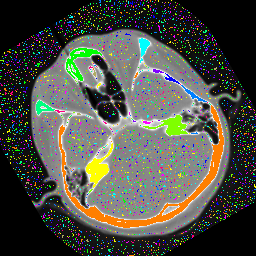
\includegraphics[scale=1]{cthead1-crmaxf}\label{fig:cthead4}}
\subfigure[FullyConnected=True]{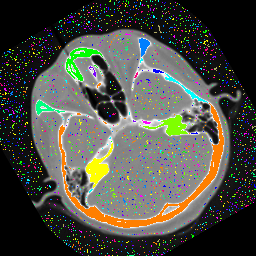
\includegraphics[scale=1]{cthead1-crmaxF}\label{fig:cthead8}}
\caption{Regional maxima of {\em cthead1} found using the flooding method with connectivity of 4 and 8.\label{fig:cthead1}}
\end{center}
\end{figure}

\section{Comparison of operations}
So which method is ``best''? Well, they are all a bit different, so
the choice will be application dependent. The labelling approach
isn't currently available as standalone filter, so it is difficult to
judge performance. The algorithm requires several steps, which may
slow it down, but some of the steps are certain to visit the pixels in
raster order, which can be a big advantage. If the regional extrema
are going to be labelled anyway then the performance may be
competitive. The reconstruction based approach is considerably slower,
but is able to do a lot more. If you are interested in image dynamics
rather than regional extrema then this is the only way to go. If you
definitely want extrema then the new filter is currently the fastest
option.

\section{Sample code}
The following code is from {\tt vrmin.cxx}, and compares the operation
of {\em ValuedRegionalMinimaImageFilter} and {\em HConcaveImageFilter}.

\small \begin{verbatim}
// a test routine for regional extrema using flooding
#include "itkValuedRegionalMinimaImageFilter.h"
#include "itkHConcaveImageFilter.h"
#include "itkMaximumImageFilter.h"
#include "itkInvertIntensityImageFilter.h"
#include "itkImageFileReader.h"
#include "itkImageFileWriter.h"
#include "itkCommand.h"
#include "itkRescaleIntensityImageFilter.h"
#include "itkAndImageFilter.h"
#include "itkCommand.h"
#include "itkSimpleFilterWatcher.h"



int main(int, char * argv[])
{
  const int dim = 2;
  
  typedef unsigned char PType;
  typedef itk::Image< PType, dim > IType;

  typedef itk::ImageFileReader< IType > ReaderType;
  ReaderType::Pointer reader = ReaderType::New();
  reader->SetFileName( argv[2] );

  typedef itk::ValuedRegionalMinimaImageFilter< IType, IType > FilterType;
  FilterType::Pointer filter = FilterType::New();
  filter->SetInput( reader->GetOutput() );
  filter->SetFullyConnected( atoi(argv[1]) );
  itk::SimpleFilterWatcher watcher(filter, "filter");

  typedef itk::ImageFileWriter< IType > WriterType;
  WriterType::Pointer writer = WriterType::New();
  writer->SetInput( filter->GetOutput() );
  writer->SetFileName( argv[3] );
  writer->Update();


  // produce the same output with other filters
  typedef itk::HConcaveImageFilter< IType, IType > ConcaveType;
  ConcaveType::Pointer concave = ConcaveType::New();
  concave->SetInput( reader->GetOutput() );
  concave->SetFullyConnected( atoi(argv[1]) );
  concave->SetHeight( 1 );

  // concave gives minima with value=1 and others with value=0
  // rescale the image so we have minima=255 other=0
  typedef itk::RescaleIntensityImageFilter< IType, IType > RescaleType;
  RescaleType::Pointer rescale = RescaleType::New();
  rescale->SetInput( concave->GetOutput() );
  rescale->SetOutputMaximum( 255 );
  rescale->SetOutputMinimum( 0 );

  // in the input image, select the values of the pixel at the minima
  typedef itk::AndImageFilter< IType, IType, IType > AndType;
  AndType::Pointer a = AndType::New();
  a->SetInput(0, rescale->GetOutput() );
  a->SetInput(1, reader->GetOutput() );

  // all pixel which are not minima must have value=255.
  // get the non minima pixel by inverting the rescaled image
  // we will have minima value=0 and non minima value=255
  typedef itk::InvertIntensityImageFilter< IType, IType > InvertType;
  InvertType::Pointer invert = InvertType::New();
  invert->SetInput( rescale->GetOutput() );

  // get the highest value from "a" and from invert. The minima have
  // value>=0 in "a" image and the non minima have a value=0. In invert,
  // the non minima have a value=255 and the minima a value=0
  typedef itk::MaximumImageFilter< IType, IType, IType > MaxType;
  MaxType::Pointer max = MaxType::New();
  max->SetInput(0, invert->GetOutput() );
  max->SetInput(1, a->GetOutput() );

  WriterType::Pointer writer2 = WriterType::New();
  writer2->SetInput( max->GetOutput() );
  writer2->SetFileName( argv[4] );
  writer2->Update();

  return 0;
}
\end{verbatim} \normalsize

\section{Acknowledgments}
We thank Dr Pierre Adenot and MIMA2 confocal facilities (\url{http://mima2.jouy.inra.fr})
for providing image samples.

\bibliographystyle{plain}
\bibliography{Article,InsightJournal}

\nocite{ITKSoftwareGuide}
\nocite{Vincent93}
\nocite{Soille2003}

\end{document}

